% Emacs settings: -*-mode: latex; TeX-master: "manual.tex"; -*-

\section{Powder sample components}
\label{powder}
In this section, we consider elastic coherent and incoherent
scattering from polycrystalline samples. We have chosen to
simulate the correct physical processes within the powder
samples on a quite detailed level.

Within many samples,
the incident beam is attenuated by scattering and absorption,
so that the illumination varies considerably throughout the sample.
For single crystals, this phenomenon is known as
{\em secondary extinction} \cite{bacon}, but the effect is
also important in powders.
In analytical treatments, attenuation is difficult to deal with,
and is thus often ignored, making a {\em thin sample approximation}.
In Monte Carlo simulations, the beam attenuation
is easily taken care of, as will be shown below.
For simplicity we ignore multiple scattering, which will
be implemented in a later version of \MCS .

\subsection{Weight transformation in samples; focusing}
Let us look in detail on how to simulate the physics of the scattering
process within the powder.
The sample has an absorption cross section per unit cell of
$\sigma_c^a$ and a scattering cross section per unit cell
of $\sigma_c^s$. The neutron path length
in the sample before the scattering event is denoted by $l_1$, and
the path length within the sample after the scattering
is denoted by $l_2$, see figure \ref{powderFig}.
We then define the inverse penetration lengths as
$\mu^s = \sigma_c^s / V_c$ and $\mu^a = \sigma_c^a / V_c$, where
$V_c$ is the volume of a unit cell. Physically, the beam
along this path is attenuated according to
\begin{equation}
P(l) = \exp(- l (\mu^s + \mu^a)) ,
\end{equation}
where the normalization is taken to be $P(0)=1$.

\begin{figure}
  \begin{center}
    \psfrag{l1}{$l_1$}
    \psfrag{l2}{$l_2$}
    \psfrag{lfull}{$l_{\rm full}$}
    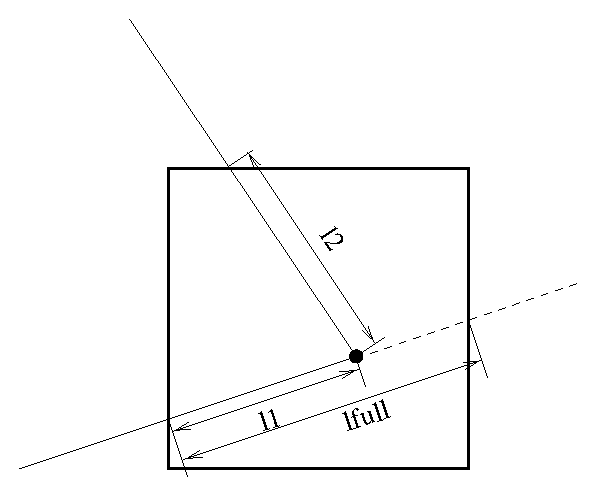
\includegraphics[width=0.6\textwidth]{figures/scatter.eps}
  \end{center}
\caption{The geometry of a scattering event within a powder sample.}
\label{powderFig}
\end{figure}

The probability for a neutron to be scattered from within the interval
$[ l_1 ; l_1+dl ]$ will be
\begin{equation}
\Pi(l_1) dl = \mu^s P(l_1) dl ,
\end{equation}
while the probability for a neutron to be scattered from within
this interval into the solid angle $\Omega$ {\em and}
not being scattered further
or absorbed on the way out of the sample is
\begin{equation}
\Pi(l_1,\Omega) dl d\Omega =
  \mu^s P(l_1) P(l_2) \gamma(\Omega) d\Omega dl ,
\end{equation}
where $\gamma(\Omega)$ is the directional distribution
of the scattered neutrons, and $l_2$ is determined by $l_1$,
$\Omega$, and the sample geometry, see figure \ref{powderFig}.

In our Monte-Carlo simulations, we will often choose the scattering
parameters by making a Monte-Carlo choice of $l_1$ and $\Omega$
from a distribution different from $\Pi(l_1,\Omega)$.
By doing this, we must adjust $\pi_i$ according to
the probability transformation rule (\ref{probrule}).
If we {\em e.g.}\ choose the scattering depth, $l_1$,
from a flat distribution in $[ 0 ; l_{\rm full} ]$,
and choose the directional dependence from $g(\Omega)$,
we have a Monte Carlo probability
\begin{equation}
f(l_1,\Omega) = g(\Omega) / l_{\rm full} ,
\end{equation}
$l_{\rm full}$ is here the path length through the sample
as taken by a non-scattered neutron (although we here
assume that all simulated neutrons are being scattered).
According to (\ref{probrule}), the neutron weight factor
is now adjusted by the amount
\begin{equation}     \label{sampleprob}
\pi_i(l_1,\Omega) =
 \mu^s l_{\rm full} \exp \left[ - (l_1+l_2) (\mu^a + \mu^s) \right]
  \frac{\gamma(\Omega)}{g(\Omega)} .
\end{equation}

In analogy with the source components, it is possible to define
interesting directions for the scattering.
One will then try to focus the scattered neutrons,
choosing a $g(\Omega)$, which peaks around these directions.
To do this, one uses (\ref{sampleprob}), where the
fraction $\gamma(\Omega)/g(\Omega)$ corrects for the focusing.
One must choose a proper distribution so that
$g(\Omega) > 0$ in every interesting direction. If this is not the
case, the Monte Carlo simulation gives incorrect results.

All samples of the powder type have been constructed with a focusing
and a non-focusing option.


\section{Powder1: A general powder sample}
\index{Samples!Powder, single diffraction line}
\index{Diffraction}
\subsection{General considerations}
An ideal powder sample consists of many small
crystallites, although each crystallite is sufficiently
large not to cause size broadening.
The orientation of the crystallites is evenly distributed,
and there is thus always a certain number of
crystallites oriented to fulfill the Bragg condition
\begin{equation}   \label{Bragg}
n \lambda = 2 d \sin \theta ,
\end{equation}
where $n$ is the order of the scattering (an integer), $\lambda$
is the neutron wavelength, $d$ is the lattice spacing of the sample,
and $2 \theta$ is the scattering angle, see figure \ref{coneFig}.
As all crystal orientations
are realised in a powder sample, the neutrons are scattered within a
{\em Debye-Scherrer cone} of opening angle $4 \theta$ \cite{bacon}.

\begin{figure}
  \begin{center}
    \psfrag{2theta}[c][c]{$2\theta$}
    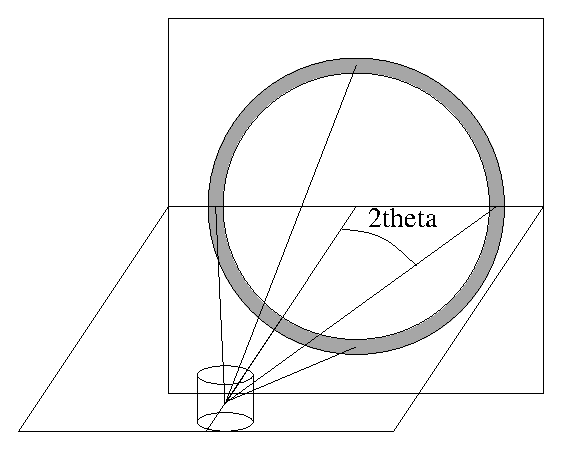
\includegraphics[width=0.6\textwidth]{figures/powder.eps}
  \end{center}
\caption{The scattering geometry of a powder sample showing the
Debye-Scherrer cone and the Debye-Scherrer circle.}
\label{coneFig}
\end{figure}

Equation (\ref{Bragg}) may be cast into the form
\begin{equation}
|{\bf Q}| = 2 |{\bf k}| \sin \theta ,
\end{equation}
where {\bf Q} is a vector of the reciprocal lattice, and {\bf k} is
the wave vector of the neutron. It is seen that only
reciprocal vectors fulfilling $|{\bf Q}| < 2 |{\bf k}|$
contribute to the scattering.
For a complete treatment of the powder sample, one needs to take
into account all these {\bf Q}-values, since each of them contribute
to the attenuation.

The textbook expression for the scattering intensity
from one reflection in a slab-shaped powder sample,
much larger than the beam cross section, reads \cite{bacon}
\begin{eqnarray}
\label{e:slab}
\frac{P}{P_0} &=& \frac{\lambda^3 l_s}{4\pi r} \frac{\rho'}{\rho}
         t j N_c^2 |F({\bf Q})|^2 \exp(-2W)
         \frac{\exp(-\mu^{\rm a} t / cos \theta)}{\sin^2(2\theta)} \\
|F({\bf Q})|^2 &=&
 \left| \sum_j b_j \exp({\bf R}_j \cdot {\bf Q}) \right|^2 ,
\end{eqnarray}
where the sum in the structure factor runs over all atoms in one unit cell.
The meanings and units of the symbols are
%
\begin{quote}\begin{tabular}{ccl}
$P_0$ & s$^{-1}$ & Incoming intensity of neutrons \\
$P$   & s$^{-1}$ & Detected intensity of neutrons \\
$l_s$ & m        & Height of detector \\
$r$   & m        & Distance from sample to detector \\
$\rho'/\rho$ & 1 & Packing factor of the powder \\
$t$   & m        & Slab thickness \\
$j$   & 1        & Multiplicity of the reflection \\
$N_c$ & m$^{-3}$ & Density of unit cells in bulk material\\
$|F({\bf Q})|^2$ & m$^2$  & Structure factor \\
$\exp(-2W)$ & 1  & Debye-Waller factor \\
$\mu^a$ & m$^{-1}$ & Linear attenuation factor due to absorption. \\
\end{tabular}\end{quote}
%
In analogy with this, the textbook expression for a cylinder shaped powder
sample, completely illuminated by the beam, reads \cite{bacon}
\begin{equation}
\frac{P}{\Psi_0} =
 \frac{V \rho'}{\rho} N_c^2 |F({\bf Q})|^2 j \exp(-2W)
                    \frac{A_{hkl}}{\sin(\theta)\sin(2\theta)}
                    \frac{l_s}{2\pi r} \frac{\lambda^3}{4} ,
\end{equation}
where the new symbols are
%
\begin{quote}\begin{tabular}{ccl}
$\Psi_0$  & s$^{-1}$m$^{-2}$ & Incoming beam flux \\
$V$       & m$^3$    & Sample volume \\
$A_{hkl}$ & 1        & Attenuation factor. \\
\end{tabular}\end{quote}
%
Eq.\ (\ref{e:slab}) for a slab shaped sample
may be cast into the form of the cylinder expression above
by using the substitutions
%
\begin{quote}\begin{tabular}{lrcl}
Incoming flux & $P_0 / (w h \cos\theta)$ & $\rightarrow$ & $\Psi_0$ \\
Sample volume & $w h t$ & $\rightarrow$ & $V$ \\
Absorption factor & $\exp(-\mu^a t / \cos\theta)$ & $\rightarrow$ & $A_{hkl}$, \\
\end{tabular}\end{quote}
%
where $h$ and $w$ are the height and width of the sample, respectively.
Often, one defines the {\em scattering power} as
\begin{equation}
Q \equiv N^2 \frac{|F({\bf Q})|^2 \lambda^3}{V \sin(2\theta)}
 = N_c^2 V \frac{\rho'}{\rho} \frac{|F({\bf Q})|^2 \lambda^3}{\sin(2\theta)} ,
\end{equation}
where $N$ is the number of unit cells.

A cut though the Debye-Scherrer cone perpendicular to its axis
is a circle. At the distance $r$ from the sample, the radius of this
circle is $r \sin(2\theta)$. Thus, the detector (in a small angle
approximation) only counts a fraction $f_d = l_s / (2 \pi r \sin(2 \theta))$
of the scattered neutrons.
One may now calculate the
linear attenuation coefficient in the material due to scattering
(from one {\bf Q}-value only):
\begin{equation}
\label{e:attenu}
\mu^s \equiv -\frac{1}{P_0} \frac{d(P/f_d)}{dl}
  = \frac{Q}{V} j \exp(-2W) \cos(\theta) .
\end{equation}
A powder sample will in general have several allowed reflections
${\bf Q}_j$, which will all contribute to the attenuation.
These reflections will have different values of
$|F({\bf Q}_j)|^2$ (and hence of $Q_j$), $j_j$, $\exp(-2W_j)$,
and $\theta_j$.
The total attenuation through the sample due to scattering is given by
$\mu^s = \mu_{\rm inc}^s + \sum_j \mu^s_j $,
where $\mu_{\rm inc}^s$ represents the incoherent scattering.

\subsection{This implementation}
For component {\bf Powder1}, we assume that the sample
has the shape of a solid cylinder.
Further, the incoherent scattering is only taken into account
by the attenuation of the beam, given by (\ref{e:attenu})
and $\sigma_c^a$.
The incoherently scattered neutrons are not
propagated through to the detector, but rather not generated at all.
Focusing is performed by only scattering into one angular
interval, $d\phi$ of the Debye-Scherrer circle. The center of this
interval is located at the point where the Debye-Scherrer circle
intersects the half-plane defined by the initial velocity, ${\bf v}_{\rm i}$,
and a user-specified vector, {\bf f}.
Multiple scattering is not implemented.

The input parameters for this component are
%
\begin{quote}\begin{tabular}{ccl}
$r$ & m & Radius of cylinder \\
$h$ & m & Height of cylinder \\
$\sigma_c^a$ & fm$^2$ & Absorption cross section per unit cell (at 2200 m/s) \\
$\sigma_{i,c}^s$ & (fm)$^2$ & Incoherent scattering cross section per unit cell \\
$\rho'/\rho$ & 1 & Packing factor \\
$V_c$ & \AA$^3$ & Volume of unit cell \\
${\bf Q}$ & \AA$^{-1}$ & The reciprocal lattice vector under consideration \\
$|F({\bf Q}_j)|^2$ & (fm)$^2$ &
 Structure factor \\
$j$ & 1 & Multiplicity of reflection \\
$\exp(-2W)$ & 1 & Debye-Waller factor \\
$d\phi$ & deg & Angular interval of focusing \\
$f_x$ & m & \\
$f_y$ & m & Focusing vector\\
$f_z$ & m & \\
\end{tabular}\end{quote}
%
The source text for the component is shown in Appendix
\ref{c:powder1}.

In a later version, more reciprocal lattice vectors will be
allowed.

